% Convolución geodésica en una variedad curva
% Compilar con: pdflatex geodesic_convolution.tex
\documentclass[tikz,border=10pt]{standalone}
\usepackage{tikz}
\usepackage{amsmath,amssymb}
\usepackage{xcolor}
\definecolor{gdlblue}{RGB}{41, 98, 168}
\definecolor{gdlred}{RGB}{191, 49, 49}
\definecolor{gdlgreen}{RGB}{30, 130, 76}
\definecolor{gdlorange}{RGB}{217, 130, 30}
\definecolor{gdlpurple}{RGB}{118, 56, 138}
\definecolor{gdlgray}{RGB}{140, 140, 140}
\definecolor{gdlyellow}{RGB}{190, 140, 10}
\usetikzlibrary{arrows.meta, decorations.markings, calc, shapes.geometric}

\begin{document}
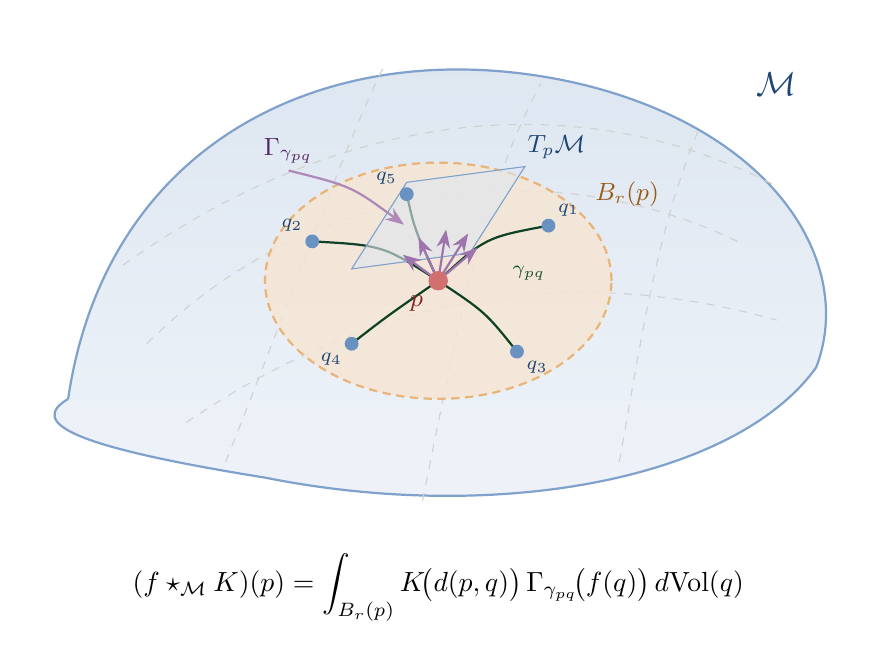
\begin{tikzpicture}[>=Stealth]

% === Superficie curva (variedad M) ===
% Forma ovalada con perspectiva 3D sugerida
\shade[top color=gdlblue!18, bottom color=gdlblue!8, opacity=0.9]
    (-4.5, -1.2) .. controls (-4, 2.2) and (-1, 3.5) .. (2, 2.8)
    .. controls (4.5, 2.2) and (5.5, 0.5) .. (5, -0.8)
    .. controls (4, -2.2) and (1, -2.8) .. (-2, -2.2)
    .. controls (-4.5, -1.8) and (-5, -1.5) .. (-4.5, -1.2);
\draw[thick, gdlblue!60]
    (-4.5, -1.2) .. controls (-4, 2.2) and (-1, 3.5) .. (2, 2.8)
    .. controls (4.5, 2.2) and (5.5, 0.5) .. (5, -0.8)
    .. controls (4, -2.2) and (1, -2.8) .. (-2, -2.2)
    .. controls (-4.5, -1.8) and (-5, -1.5) .. (-4.5, -1.2);

% Líneas de malla (mesh) para sugerir curvatura
\draw[gdlgray!40, dashed]
    (-3.5, -0.5) .. controls (-1.5, 1.5) and (1.5, 2) .. (4, 0.8);
\draw[gdlgray!40, dashed]
    (-3.8, 0.5) .. controls (-1, 2.5) and (2, 2.8) .. (4.5, 1.5);
\draw[gdlgray!40, dashed]
    (-3, -1.5) .. controls (-0.5, 0.2) and (2, 0.5) .. (4.5, -0.2);
\draw[gdlgray!40, dashed]
    (-2.5, -2) .. controls (-1.5, 0.5) and (-1, 2) .. (-0.5, 3);
\draw[gdlgray!40, dashed]
    (0, -2.5) .. controls (0.5, 0) and (0.8, 1.5) .. (1.5, 2.8);
\draw[gdlgray!40, dashed]
    (2.5, -2) .. controls (2.8, -0.3) and (3, 1) .. (3.5, 2.2);

% Etiqueta de la variedad
\node[gdlblue!70!black, font=\large] at (4.5, 2.8) {$\mathcal{M}$};

% === Bola geodésica B_r(p) ===
% Región sombreada elíptica (perspectiva) alrededor de p
\fill[gdlorange!20, opacity=0.8]
    (0.2, 0.3) ellipse (2.2cm and 1.5cm);
\draw[thick, gdlorange!60, densely dashed]
    (0.2, 0.3) ellipse (2.2cm and 1.5cm);

% Etiqueta de la bola geodésica
\node[gdlorange!70!black, font=\small] at (2.6, 1.4) {$B_r(p)$};

% === Punto central p ===
\coordinate (p) at (0.2, 0.3);

% === Puntos vecinos q_j dentro de la bola ===
\coordinate (q1) at (1.6, 1.0);
\coordinate (q2) at (-1.4, 0.8);
\coordinate (q3) at (1.2, -0.6);
\coordinate (q4) at (-0.9, -0.5);
\coordinate (q5) at (-0.2, 1.4);

% === Geodésicas de p a q_j (detrás de todo lo demás) ===
\draw[thick, gdlgreen!50!black]
    (p) .. controls (0.8, 0.85) .. (q1);
\draw[thick, gdlgreen!50!black]
    (p) .. controls (-0.5, 0.75) .. (q2);
\draw[thick, gdlgreen!50!black]
    (p) .. controls (0.8, -0.1) .. (q3);
\draw[thick, gdlgreen!50!black]
    (p) .. controls (-0.45, -0.15) .. (q4);
\draw[thick, gdlgreen!50!black]
    (p) .. controls (-0.1, 0.95) .. (q5);

% Etiqueta de una geodésica representativa
\node[gdlgreen!60!black, font=\scriptsize] at (1.35, 0.4) {$\gamma_{pq}$};

% === Plano tangente T_pM ===
% Paralelogramo inclinado más compacto, ligeramente elevado
\fill[gdlblue!15, opacity=0.6]
    ([shift={(-1.1, 0.15)}] p) --
    ([shift={(-0.4, 1.25)}] p) --
    ([shift={(1.1, 1.45)}] p) --
    ([shift={(0.4, 0.35)}] p) -- cycle;
\draw[gdlblue!60]
    ([shift={(-1.1, 0.15)}] p) --
    ([shift={(-0.4, 1.25)}] p) --
    ([shift={(1.1, 1.45)}] p) --
    ([shift={(0.4, 0.35)}] p) -- cycle;

% Etiqueta del plano tangente
\node[gdlblue!70!black, font=\small] at (1.7, 2.0) {$T_p\mathcal{M}$};

% === Vectores transportados (flechas en T_pM) ===
% Vectores f(q_j) transportados paralelamente a p via Gamma_{gamma_{pq}}
\draw[->, thick, gdlpurple!70] (p) -- ++(0.5, 0.42);
\draw[->, thick, gdlpurple!70] (p) -- ++(-0.45, 0.33);
\draw[->, thick, gdlpurple!70] (p) -- ++(0.38, 0.6);
\draw[->, thick, gdlpurple!70] (p) -- ++(-0.25, 0.55);
\draw[->, thick, gdlpurple!70] (p) -- ++(0.1, 0.65);

% Etiqueta del transporte paralelo (junto a un vector representativo)
\draw[->, gdlpurple!60, thick, shorten >=3pt]
    (-1.7, 1.7) .. controls (-0.9, 1.5) .. (-0.15, 0.95);
\node[gdlpurple!70!black, font=\small] at (-1.7, 1.95) {$\Gamma_{\gamma_{pq}}$};

% === Puntos q_j (encima de geodésicas) ===
\fill[gdlblue!70] (q1) circle (2.5pt);
\fill[gdlblue!70] (q2) circle (2.5pt);
\fill[gdlblue!70] (q3) circle (2.5pt);
\fill[gdlblue!70] (q4) circle (2.5pt);
\fill[gdlblue!70] (q5) circle (2.5pt);

% Etiquetas q_j
\node[above right, gdlblue!70!black, font=\scriptsize] at (q1) {$q_1$};
\node[above left, gdlblue!70!black, font=\scriptsize] at (q2) {$q_2$};
\node[below right, gdlblue!70!black, font=\scriptsize] at (q3) {$q_3$};
\node[below left, gdlblue!70!black, font=\scriptsize] at (q4) {$q_4$};
\node[above left, gdlblue!70!black, font=\scriptsize] at (q5) {$q_5$};

% === Punto p encima de todo ===
\fill[gdlred!70] (p) circle (3.5pt);
\node[below left=2pt, gdlred!70!black, font=\small] at (p) {$p$};

% === Fórmula de convolución geodésica ===
\node[font=\normalsize, text=black] at (0.2, -3.6) {%
    $\displaystyle (f \star_{\mathcal{M}} K)(p)
    = \int_{B_r(p)} K\!\bigl(d(p,q)\bigr)\,
    \Gamma_{\gamma_{pq}}\!\bigl(f(q)\bigr)\, d\mathrm{Vol}(q)$%
};

\end{tikzpicture}
\end{document}
